\documentclass[tikz,border=8pt]{standalone}
% Shared look for every TikZ diagram. Load with \input{../../tools/tikz-style.tex}
\usepackage[sfdefault]{roboto}
\usetikzlibrary{arrows.meta, positioning, shapes.geometric, calc, fit, backgrounds}
\definecolor{cblue}{HTML}{4C78A8}
\definecolor{corange}{HTML}{F58518}
\definecolor{cgreen}{HTML}{54A24B}
\definecolor{cred}{HTML}{E45756}
\definecolor{cpurple}{HTML}{B279A2}
\definecolor{cgrey}{HTML}{6B6B6B}
\tikzset{
  every picture/.style={font=\sffamily, line width=1.2pt},
  box/.style={draw=#1, fill=#1!12, rounded corners=4pt, align=center, inner sep=7pt, minimum height=1.1cm},
  box/.default=cgrey,
  arrow/.style={-{Stealth[length=3mm]}, draw=cgrey, line width=1.4pt},
  title/.style={font=\sffamily\bfseries\Large},
  note/.style={font=\sffamily\small, text=cgrey, align=center},
}
\AtBeginDocument{\hyphenpenalty=10000 \exhyphenpenalty=10000}

% Left: the node kinds of a behaviour tree and their symbols (Colledanchise and Ogren, ch. 1, Table 1.1).
% Right: the smallest navigation tree, with the answers of its first tick at t = 0.00 s (notebook): ticks go down,
% answers come up.
\begin{document}
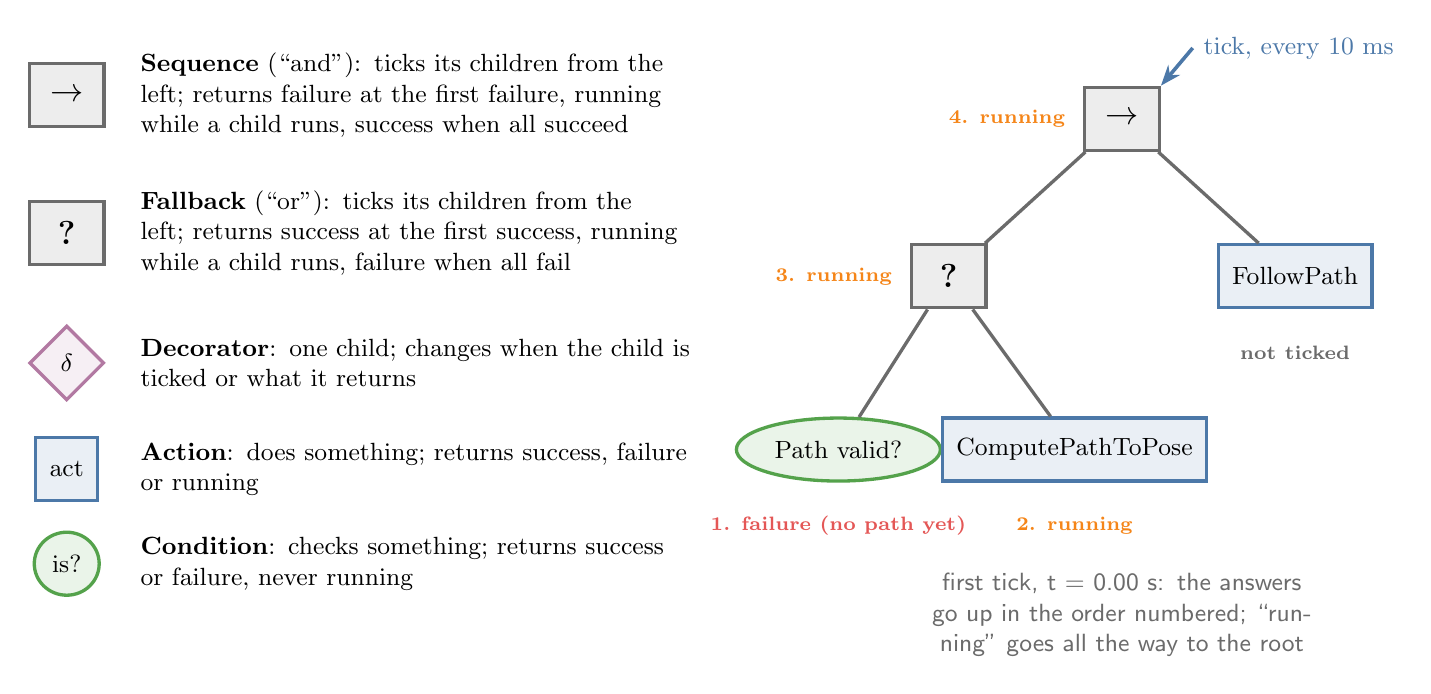
\begin{tikzpicture}[
  ctl/.style={draw=cgrey, fill=cgrey!12, minimum width=0.95cm, minimum height=0.8cm, font=\large\bfseries},
  act/.style={draw=cblue, fill=cblue!12, minimum height=0.8cm, inner sep=5pt, font=\small},
  cnd/.style={ellipse, draw=cgreen, fill=cgreen!12, minimum height=0.8cm, inner sep=3pt, font=\small},
  dec/.style={diamond, draw=cpurple, fill=cpurple!12, minimum size=0.95cm, inner sep=1pt, font=\small},
  rule/.style={font=\small, anchor=west, text width=7.0cm, align=left},
  ans/.style={font=\scriptsize\bfseries, fill=white, inner sep=1.5pt},
  edge/.style={draw=cgrey, line width=1.2pt}]
  % the legend
  \node[ctl] (l1) at (0,0) {$\rightarrow$};
  \node[rule] at (0.8,0) {\textbf{Sequence} (``and''): ticks its children from the left; returns failure at the first failure, running while a child runs, success when all succeed};
  \node[ctl] (l2) at (0,-1.75) {?};
  \node[rule] at (0.8,-1.75) {\textbf{Fallback} (``or''): ticks its children from the left; returns success at the first success, running while a child runs, failure when all fail};
  \node[dec] (l3) at (0,-3.4) {$\delta$};
  \node[rule] at (0.8,-3.4) {\textbf{Decorator}: one child; changes when the child is ticked or what it returns};
  \node[act] (l4) at (0,-4.75) {act};
  \node[rule] at (0.8,-4.75) {\textbf{Action}: does something; returns success, failure or running};
  \node[cnd] (l5) at (0,-5.95) {is?};
  \node[rule] at (0.8,-5.95) {\textbf{Condition}: checks something; returns success or failure, never running};
  % the small tree at its first tick
  \begin{scope}[xshift=13.4cm, yshift=-0.3cm]
    \node[ctl] (root) at (0,0) {$\rightarrow$};
    \node[ctl] (fb) at (-2.2,-2.0) {?};
    \node[act] (fp) at (2.2,-2.0) {FollowPath};
    \node[cnd] (pv) at (-3.6,-4.2) {Path valid?};
    \node[act] (cp) at (-0.6,-4.2) {ComputePathToPose};
    \draw[edge] (root) -- (fb); \draw[edge] (root) -- (fp);
    \draw[edge] (fb) -- (pv); \draw[edge] (fb) -- (cp);
    \node[ans, text=cred] at ([yshift=-0.55cm]pv.south) {1. failure (no path yet)};
    \node[ans, text=corange] at ([yshift=-0.55cm]cp.south) {2. running};
    \node[ans, text=corange, anchor=east] at ([xshift=-0.15cm]fb.west) {3. running};
    \node[ans, text=corange, anchor=east] at ([xshift=-0.15cm]root.west) {4. running};
    \node[ans, text=cgrey] at ([yshift=-0.55cm]fp.south) {not ticked};
    \draw[-{Stealth[length=2.6mm]}, draw=cblue, line width=1.3pt] (0.9,0.9) node[right, font=\small, text=cblue] {tick, every 10 ms} -- (root.north east);
    \node[note, text width=5.4cm] at (0,-6.3) {first tick, t = 0.00 s: the answers go up in the order numbered; ``running'' goes all the way to the root};
  \end{scope}
\end{tikzpicture}
\end{document}
